%
%{{{ misc

\documentclass{acmsiggraph}               % final
%\documentclass[review]{acmsiggraph}      % review
%\documentclass[widereview]{acmsiggraph}  % wide-spaced review
%\documentclass[preprint]{acmsiggraph}    % preprint

% Uncomment one of the four lines above depending on where your paper is
% in the conference process. ``review'' and ``widereview'' are for review
% submission, ``preprint'' is for pre-publication, and ``final'' is for
% the version to be printed.

% Quote:
%\usepackage[english]{babel}
\usepackage[utf8]{inputenc} % this is needed for umlauts
\usepackage[english]{babel} % this is needed for umlauts
\usepackage[T1]{fontenc}    % this is needed for correct output of umlauts in pdf
\usepackage{lmodern}
% \usepackage[fixlanguage]{babelbib}
% \selectbiblanguage{german}

\usepackage{amssymb}
\usepackage{multirow}
\usepackage{enumerate}
\usepackage{mathtools}
\usepackage{mathptmx}
\usepackage{graphicx}
\usepackage{epstopdf}
\usepackage{subcaption}

% use this for zero \parindent and non-zero \parskip, intelligently.

\usepackage{parskip}
\usepackage{enumitem}
\usepackage{booktabs}
\usepackage{array}
\usepackage[official]{eurosym} % euro with \euro{} command
\usepackage[page]{appendix}

%Peseudocode
\usepackage{algpseudocode}
\usepackage{algorithm}
%Fancy shit
\usepackage{url}

\usepackage[pdftitle={Proposal on Investigating Media Transparency},
            pdfauthor={David Pfahler},
            pdfsubject={Praktikum aus Visual Computing},
            pdfborder={0 0 0}]{hyperref}

% If you are submitting a paper to the annual conference, please replace 
% the value ``0'' below with your OnlineID. If you are not submitting this
% paper to the annual conference, you may safely leave it at ``0'' -- it 
% will not be included in the output.

\onlineid{0}

% need to document this!

\acmformat{print}

% Paper title.

\title{\fontsize{12}{12pt} \bf 188.943 Praktikum aus Visual Computing
  ~\\[0.5cm]
  \fontsize{14}{14pt} \bf Proposal on Investigating Media Transparency
  ~\\[0.5cm]
  \fontsize{12}{12pt} \bf \today}

% Author and Affiliation (single author).

%\author{Roy G. Biv\thanks{e-mail: roy.g.biv@aol.com}\\Allied Widgets Research}

% Author and Affiliation (multiple authors).

\author{David Pfahler\thanks{e-mail: e1126287@student.tuwien.ac.at}\\ TU Wien, Austria %
\and Supervisor: Alexander Rind\thanks{e-mail: alexander.rind@fhstp.ac.at}\\ St. P{\"o}lten University of Applied Sciences %
\and Supervisor: Wolfgang Aigner\thanks{e-mail: alexander.rind@fhstp.ac.at}\\ TU Wien, Information Engineering Group, Austria
}

% Keywords that describe your work.

\keywords{Visual Analytics, Data Driven Journalism, Media Transparency, Politics, Journalism, Network, Time-Oriented-Data}

\makeatletter
\def\thebibliography#1{%
  \section*{%
    \refname\@mkboth{\sl\uppercase{\refname}}{\sl\uppercase{\refname}}}
  \list{\@biblabel{\@arabic\c@enumiv}}{%
            \settowidth\labelwidth{\@biblabel{#1}}%
            \leftmargin\labelwidth%
            \advance\leftmargin\labelsep%
            \@openbib@code%
            \usecounter{enumiv}%
            \let\p@enumiv\@empty%
            \renewcommand\theenumiv{\@arabic\c@enumiv}%
            \setlength{\labelsep}{0em}}
  \def\newblock{\hskip .11em plus .33em minus .07em}%
  \sloppy\clubpenalty4000\widowpenalty4000%
  \sfcode`\.=1000\relax}
\def\@biblabel#1{\hspace*{-.5pc}[#1]\hspace*{.5pc}}

% START OF THE PAPER %

\begin{document}

% The ``\maketitle'' command must be the first command after the
% ``\begin{document}'' command. It prepares and prints the title block.

\teaser{
  \begin{subfigure}{0.45\linewidth}
    \centering
      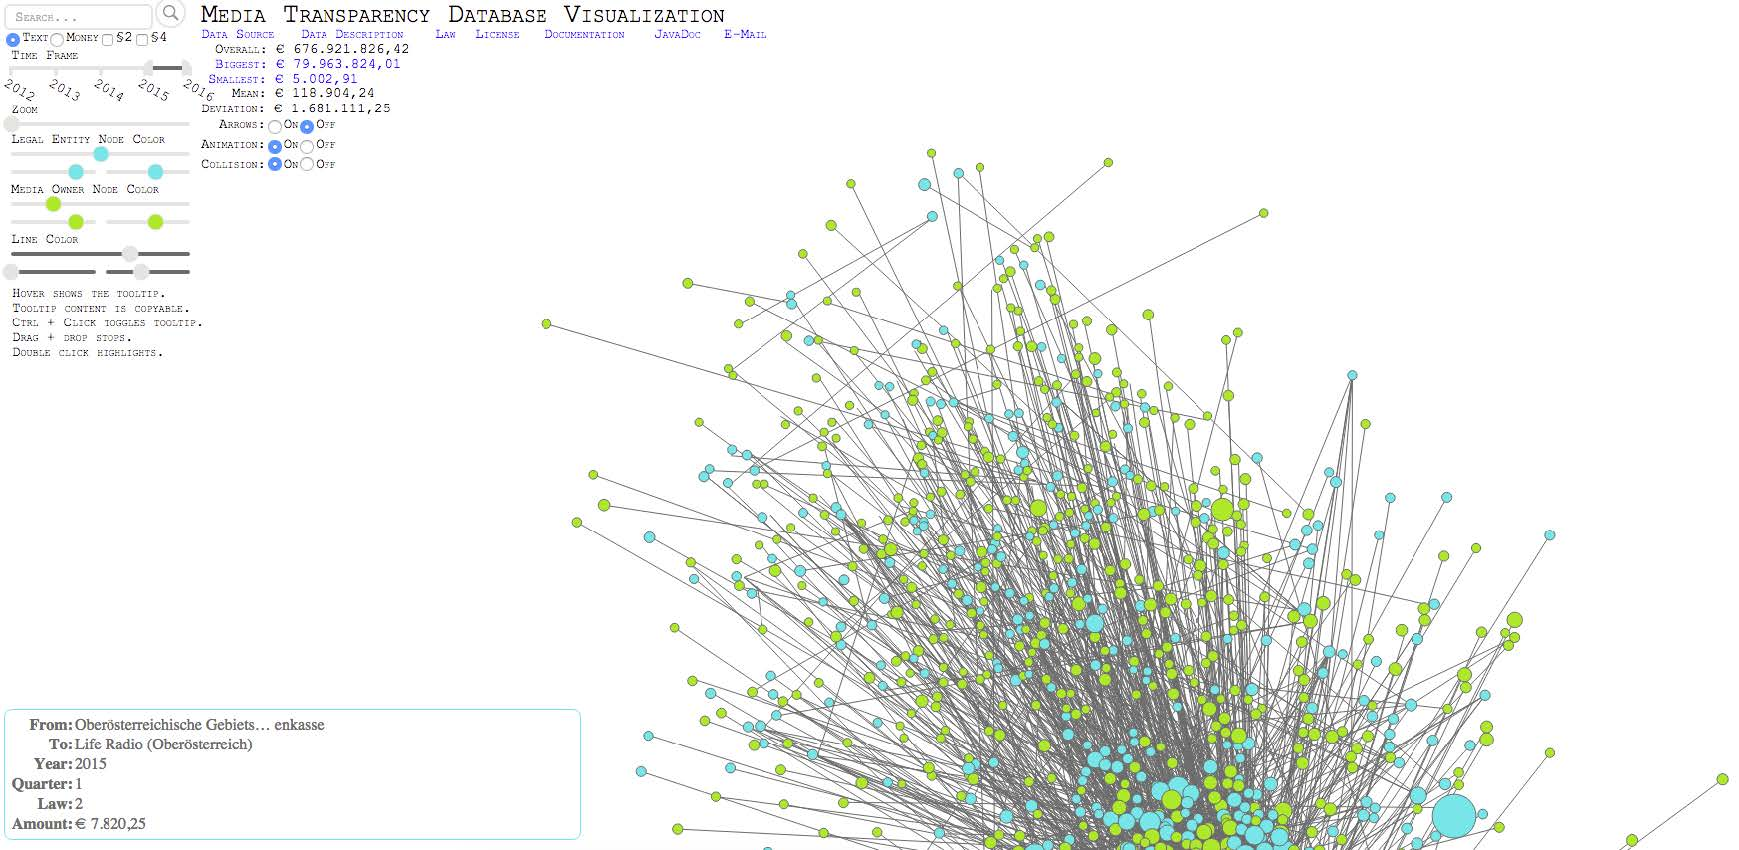
\includegraphics[height=2in]{img/forcedirected.jpg}
      \caption{}
      \label{fig:forcedirected}
  \end{subfigure}
  ~
  %add desired spacing between images, e. g. ~, \quad, \qquad, \hfill etc.
  %(or a blank line to force the subfigure onto a new line)
  \begin{subfigure}{0.45\linewidth}
    \centering
    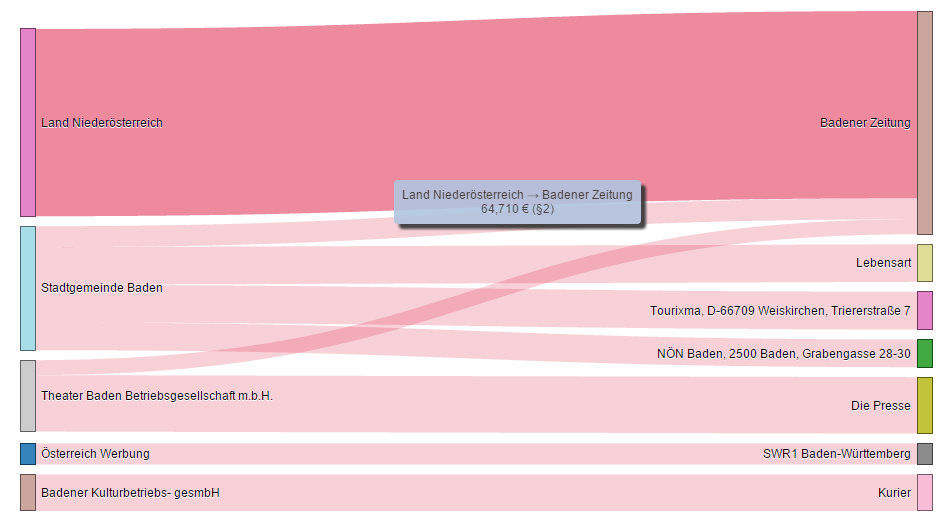
\includegraphics[height=2in]{img/BadenFilter.png}
    \caption{}
    \label{fig:badenfilter}
  \end{subfigure}%
  \caption{Screenshots of (\ref{fig:forcedirected}) a force directed node link diagram. \protect\cite{Schrempf2014} and (\ref{fig:badenfilter}) a payment flow visualization filtered by the keyword: ``Baden''. \protect\cite{fhMedien}}
  \label{fig:relatedwork}
}

\maketitle

% Abstract section.

\begin{abstract}

% State the problem
The ``media transparency database'' contains the accumulated amount of money spent by governmental organizations on media companies. This data can be explored as a multimodal dynamic network. 
% Say why it's an interesting problem
Existing web projects already present solutions to visualize the dataset, but to analyse the data further a user needs more interaction methods.
% Say what your solution achieves
I am going to implement a task-tailored dashboard with multiple connected views, which implement brushing and linking to enable the user to analyse the dataset in an easy to use matter.  
% Say what follows from your solution


\end{abstract}

% ACM Computing Review (CR) categories. 
% See <http://www.acm.org/class/1998/> for details.
% The ``\CRcat'' command takes four arguments.

% \begin{CRcatlist}
%   \CRcat{K.6.1}{Management of Computing and Information Systems}%
% {Project and People Management}{Life Cycle};
%   \CRcat{K.7.m}{The Computing Profession}{Miscellaneous}{Ethics}
% \end{CRcatlist}

% The ``\keywordlist'' command prints out the keywords.
\keywordlist


\section{Problem Description}

% The ``\copyrightspace'' command must be the first command after the 
% start of the first section of the body of your paper. It ensures the
% copyright space is left at the bottom of the first column on the first
% page of your paper.

\copyrightspace

Governmental advertisement in media and sponsorships are a possible way to influence press opinion. Therefore, the Austrian parliament passed a law that made it mandatory for governmental organizations to disclose their expenses for advertisements in different media (TV, radio, print, as well as online) \cite{Gesetz}.
\par
This so-called ``media transparency database'' is made publicly available by the Austrian Regulatory Authority for Broadcasting and Telecommunications (RTR) via the Austrian open government data portal \cite{RTR}.
It contains the accumulated amount of money transferred in a certain quarter of the year for each governmental organization and media company. This database can be explored as a multimodal dynamic network.
\par
During the project I want to implement an interactive visual analytics dashboard to explore the media transparency database efficiently. 
\par
In Section~\ref{sec:related_work} previous approaches of visualizing the database are presented. In Section~\ref{sec:expected_results} I present the expected results of my approach and in Section~\ref{sec:method} the used methods and the technologies are described.

\subsection{Data Structure} % (fold)
\label{sub:data_description}

\begin{table*}[!htb]
  \begin{center}
    \begin{tabular}{lrrlr}
    \toprule
    Rechtstr{\"a}ger&Jahr Quartal&Gesetz&Medium&Euro\\
    \midrule
    Abfallwirtschaft Tirol-Mitte GesmbH&2012 Q4&§2&Bezirksblätter Tirol &8.122,32~\euro\\
    Agrarmarkt Austria Marketing GesmbH&2012 Q4&§2&Falstaff&26.418,00~\euro\\
    Agrarmarkt Austria Marketing GesmbH&2012 Q4&§2&Connoisseur Circle&6.142,50~\euro\\
    Agrarmarkt Austria Marketing GesmbH&2012 Q4&§2&bz-Wiener Bezirkszeitung&7.031,16~\euro\\
    \multicolumn{4}{c}{$\vdots$}
    \end{tabular}
  \end{center}
  \caption{The first 4 entries of the ``media transparency database''}
  \label{tab:data}
\end{table*}

\begin{table}[!htb]
  \begin{center}
    \begin{tabular}{lrr}
    \toprule
    Media&Number of relations&Sum\\
    \midrule
    Kronen Zeitung&1042&47.748.890,86~\euro\\
    KRONE&15&2.524.123,07~\euro\\
    Kronehit&172&2.223.498,63~\euro\\
    Kronen Zeitung&1&1.387.919,29~\euro\\
    Krone bunt&26&1.193.156,45~\euro\\
    Kronen Zeitung&1&1.071.461,24~\euro\\
    Krone&25&585.228,77~\euro\\
    www.krone.at&49&524.306,82~\euro\\
    KRONEHIT&42&479.324,52~\euro\\
    \multicolumn{3}{c}{$\vdots$}
    \end{tabular}
  \end{center}
  \caption{The first entries of the ``media transparency database'' filtered by the query string for the media entries ``Krone'' ordered by the sum of the amount of transfered money}
  \label{tab:krone}
\end{table}

The media transparency database is structured as a Table with each row containing a relation from one governmental organization (\emph{Rechtstr{\"a}ger}) to one media company (\emph{Medium}). This relation contains the amount of transfered money (\emph{Euro}), the quarter of the year (\emph{Jahr Quartal}) and the law of the reason of the payment (\emph{Gesetz}). Table~\ref{tab:data} shows the first four entries of this table. 
\par
The table contains over 145000 entries over 12 quarters. So that one quarter contains 13000 data entries. There are over 1000 governmental organizations and media companies.
\par
The data quality of the database is not sufficient enough for some data entries. These entries include spelling mistakes or are just differently formated. Table~\ref{tab:krone} shows the data quality problems of this database on the example of the different entries of the media company ``Kronen Zeitung''.

% subsection data_description (end)

\section{Related Work} % (fold)
\label{sec:related_work}

The ``media transparency database'' is available since the third quarter of 2012. Since then several visualizations got presented:
\begin{itemize}
  \item \cite{paroli2} presents a visualization that uses grouping of the media entities to reduce the screen space and complexity of the visualization. It only uses one quarter of one year of the total data. It is possible to interact with the visualization and ungroup the media entities.
  \item \cite{standard} presents a static visualization with bar charts and a line plot as a visualization for time oriented data by the Austrian newspaper ``Der Standard''.
  \item One of my colleagues implemented a force directed node link diagram. The user of this visualization is able to interact with the data and filter it with different queries. But the force directed node link diagram was too slow for the huge database \cite{Schrempf2014}. 
  \item \cite{fhMedien} implemented a website to get an overview of the media dataset. It features multiple visualizations which are all interactive but not connected to one dashboard.
\end{itemize}
The first two visualizations are presentations of an analysis of the data. But the last two approaches are visualizations that support the user to analyze and investigate into the data. The force directed node link diagram has the problem that it is too slow to render a nice overview of the dynamic network. Additionally it is hard to interpret the payment flow, because it is visually encoded in the size of the nodes of the diagram. Figure~\ref{fig:forcedirected} shows the node link diagram with too many nodes.
\par
The visualization of \cite{fhMedien} is stable, easy and fast to interact. But the visualizations are distributed onto 4 different web pages, which makes it hard to combine the insight of the user from one visualization with the others. Additionally the payment flow visualization is restricted to only 800 relations. Figure~\ref{fig:badenfilter} shows the payment flow for the filter with the keyword ``Baden''.
 
% section related_work (end)

\section{Expected Results} % (fold)
\label{sec:expected_results}

My approach to improve the previously implemented visualizations is to combine multiple visualizations into a task-tailored visual analytics dashboard \cite{PB-VRVis-2014-028} and combine them with linking and brushing \cite{Ahlberg1994}.
\par
With this designed interface the information is more structured and in an easy to read manner~\cite{Elias2011}.

% section expected_results (end)

\subsection{Multiple Views} % (fold)
\label{sub:multiple_views}

The main contribution of my project is the connection of multiple views into one task tailored dashboard. This dashboard should give the user the possibility of gaining an overview of the data, but also explore details of the dataset to gain insight.
\par
The following views are going to be implemented:

\begin{description}
  \item[Aggregation] A part of the dashboard is used to aggregate the data to visualize an overview of the currently selected data. For example bar charts are used to visualize the money flow in the selected years or quarters. Additionally this views enables the user to create a high level selection, for example on a specific year or quarter.
  \item[Flow] The visualization of the cash flow of a legal entity to its media entities has to be encoded with a flow visualization. (see Subsection~\ref{sub:flow_visualization})
  \item[Details] the details of the selected entries are displayed by visualizations on demand and with a table of the entries.
\end{description}

% subsection multiple_views (end)

\subsection{Flow Visualization} % (fold)
\label{sub:flow_visualization}

In the context of this ``media transparency database'' a survey was created, which compared different network flow representations. \cite{survey} The results of this survey showed that all representations used combinations of existing techniques based on the node-link diagram and 5 of 6 online visualization techniques were based on sankey- or chord diagrams. \par
Based on this results I am going to implement a chord diagram to visualize the flow network data of the database.

% subsection flow_visualization (end)

\subsection{Data Wrangling} % (fold)
\label{sub:data_wrangling}

In Section~\ref{sub:data_description} the problem of the data quality is presented. To enhance this data quality it is necessary to edit the data before visualizing it. I want to include simple data wrangling techniques. \cite{Kandel2011} This includes joining a set of legal entries or media entries into one, while retaining the relations and removing a set of entries from the visualized data, including its relations.

% subsection data_wrangling (end)

\subsection{Interactions} % (fold)
\label{sub:interactions}

The interaction with the visualizations is essential for the user to explore the data and to verify or deny a created hypothesis. The user should be able to:

\begin{description}
  \item[Filter/Sort] for time and money.
  \item[Search] for nodes. Which are legal and media entities.
  \item[Combine and remove] a selection. (See Subsection~\ref{sub:data_wrangling})
  \item[Select] entries to get insight into this entry with brushing and linking. 
\end{description}

% subsection interactions (end)

\section{Methods} % (fold)
\label{sec:method}

In this Section I present how I want to create and design the media transparency dashboard. \par
My ideas of the design, the used visualizations and interaction techniques were inspired by the related work (see Section~\ref{sec:related_work}. Additionally I held feedback with my supervisor and experimented with the data in existing visualizations in diverse technologies like Visplore \cite{Piringer2009} or Tableau \cite{tableau}. The used technologies are presented in Subsection~\ref{sub:technologies} and the software quality assurance plan is presented in Subsection~\ref{sub:software_quality_assurance_plan}.
% section method (end)

\subsection{Technologies} % (fold)
\label{sub:technologies}

The following technologies are going to be used:
\begin{description}
  \item[JavaScript] a script language to create dynamic client side webpage.
  \item[Data-Driven Documents] A JavaScript library for manipulating documents based on data.\cite{D3}
  \item[jQuery] A fast, small, and feature-rich JavaScript library.\cite{jQ}
  \item[Bootstrap] A framework for developing responsive, mobile first projects on the web.\cite{BS}
  \item[Brunch] A node.js \cite{node} build tool to compile scripts and styles and to concatenate scripts and styles. \cite{brunsh}
  \item[clean-css] Is a node.js \cite{node} library for minifying CSS files.
  \item[uglify-js] Is a node.js \cite{node} library for minifying JavaScript files.
  \item[crossfilter] Is a JavaScript library to explore multivariate datasets with coordinated views. \cite{crossfilter}
  \item[DC] Is a JavaScript library with native crossfilter support to create charts for multidimensional data exploration\cite{dc} 
  \item[Git] Is used as version control system. 
\end{description}
% subsection technologies (end)

\subsection{software quality assurance plan} % (fold)
\label{sub:software_quality_assurance_plan}

To ensure the quality of the software I am going to test the software in the three most common used browsers. \cite{browserStatistics}
\begin{itemize}
  \item Chrome (68.4\%): From Version C 45 (2.3\%)
  \item Firefox (19.2\%): From Version FF41 (4.2\%)
  \item Internet Explorer (6.8\%):  In Edge (1.0\%) and IE 11 (4.4\%) 
\end{itemize}

Additionally I am going to make an usability expert review with my Supervisor or Christina Niederer and to ensure that the software is also usable by non expert users I am going to make informal usability tests with users who have no experience with information visualization or computer science.

% subsection software_quality_assurance_plan (end)

\bibliographystyle{abbrv}
\bibliography{bibliography}

\begin{appendices}

\section{Work Packages}

\begin{figure*}[tb]
\centering
  \begin{subfigure}{0.6\linewidth}
    \centering
      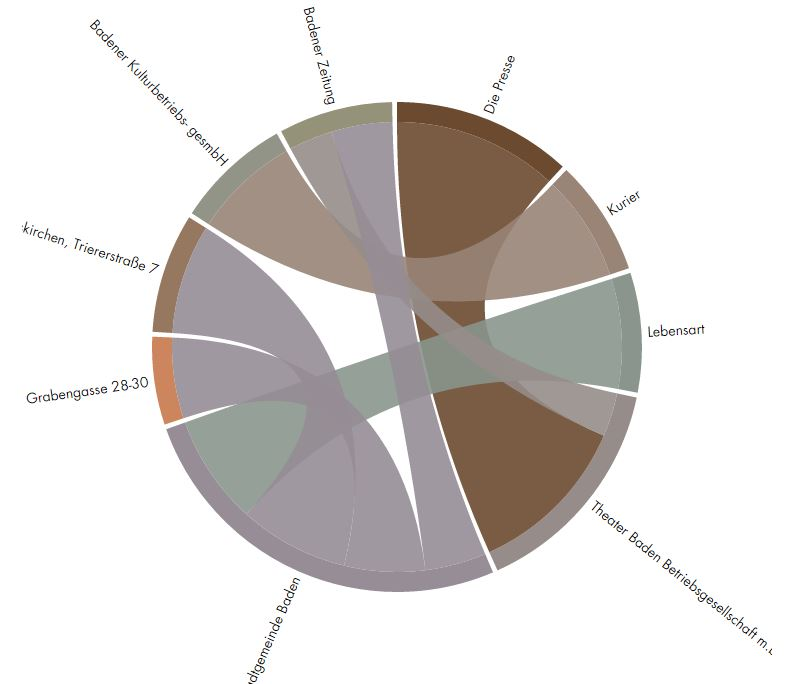
\includegraphics[width=\linewidth]{img/flowviz.jpg}
      \caption{A chord diagram}
      \label{fig:flowviz}
  \end{subfigure}
  
  \begin{subfigure}{0.45\linewidth}
    \centering
      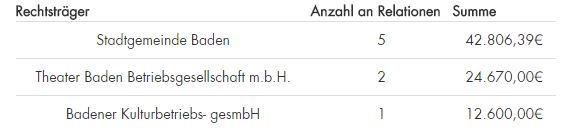
\includegraphics[width=\linewidth]{img/badentable.jpg}
      \caption{A table to browse details}
      \label{fig:table}
  \end{subfigure}   
  ~
  \begin{subfigure}{0.45\linewidth}
    \centering
      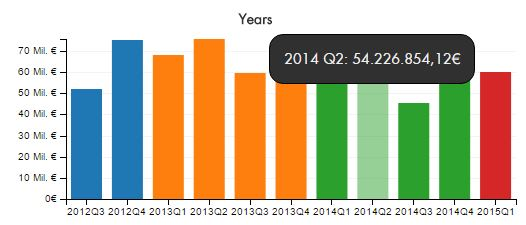
\includegraphics[width=\linewidth]{img/details.jpg}
      \caption{Details on demand on a filter visualization}
      \label{fig:details}
  \end{subfigure}

  \begin{subfigure}{0.9\linewidth}
    \centering
      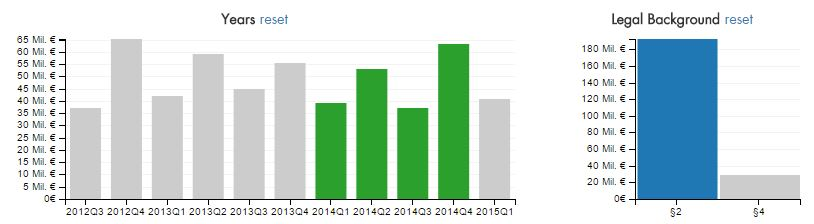
\includegraphics[width=\linewidth]{img/selection.jpg}
      \caption{A selection on one year and on one legal background}
      \label{fig:selection}
  \end{subfigure}    
\label{fig:work packages}
\end{figure*}

\subsection{Flow Visualization}

This diagram is going to visualize the money flow from governmental organizations to the media companies and is therefore a key feature. Figure~\ref{fig:flowviz} shows a first prototype of a flow visualization and is already a expected result.

\subsection{Filter Charts}

The filtering should be done partly as direct interaction with diagrams. Therefore bar charts or pie charts for ordinal data structures are a good visualization technique. Figure~\ref{fig:details} shows a bar chart of the money flow over the last years. One bar is hovered with the mouse and details on demand are displayed as a tooltip. In Figure~\ref{fig:selection} a selection on one year and on one legal background is done by interacting directly with the visualization in the dashboard.

\subsection{Detail Visualization}

To explore and browse the data it is also necessary to visualize the details of the data. This is done by detail on demand (see Figure~\ref{fig:details}) but also with a data table (see Figure~\ref{fig:table})

\subsection{Interaction}

Different interaction techniques are needed to analyse the data. They are presented in the Section~\ref{sub:interactions}.

\section{Time Plan}

\begin{description}
  \item[23.12.2015] The first prototype is up and running. All features from the work packages are at least partly implemented or mocked to get an impression on how the finished application will work. It should only run on the Chrome Browser. So it is possible to get feedback from the supervisor.
  \item[22.01.2016] The project is finished and tested on the three major browsers. The usability expert review and the informal usability tests are going to be made and the results get included into the presentation.
  \item[29.01.2016] The presentation of the project.
\end{description}

\end{appendices}

\end{document}
